% !TEX encoding = UTF-8 Unicode
\documentclass[a4paper]{article}

\usepackage{color}
\usepackage{url}
\usepackage[T2A]{fontenc} % enable Cyrillic fonts
\usepackage[utf8]{inputenc} % make weird characters work
\usepackage{graphicx}
\usepackage{float}
\usepackage{enumitem}

\usepackage[english,serbian]{babel}
%\usepackage[english,serbianc]{babel} %ukljuciti babel sa ovim opcijama, umesto gornjim, ukoliko se koristi cirilica

\usepackage[unicode]{hyperref}
\hypersetup{colorlinks,citecolor=green,filecolor=green,linkcolor=blue,urlcolor=blue}

\usepackage{listings}

%\newtheorem{primer}{Пример}[section] %ćirilični primer
\newtheorem{primer}{Primer}[section]

\definecolor{mygreen}{rgb}{0,0.6,0}
\definecolor{mygray}{rgb}{0.5,0.5,0.5}
\definecolor{mymauve}{rgb}{0.58,0,0.82}

\lstset{ 
  backgroundcolor=\color{white},   % choose the background color; you must add \usepackage{color} or \usepackage{xcolor}; should come as last argument
  basicstyle=\scriptsize\ttfamily,        % the size of the fonts that are used for the code
  breakatwhitespace=false,         % sets if automatic breaks should only happen at whitespace
  breaklines=true,                 % sets automatic line breaking
  captionpos=b,                    % sets the caption-position to bottom
  commentstyle=\color{mygreen},    % comment style
  deletekeywords={...},            % if you want to delete keywords from the given language
  escapeinside={\%*}{*)},          % if you want to add LaTeX within your code
  extendedchars=true,              % lets you use non-ASCII characters; for 8-bits encodings only, does not work with UTF-8
  firstnumber=1000,                % start line enumeration with line 1000
  frame=single,	                   % adds a frame around the code
  keepspaces=true,                 % keeps spaces in text, useful for keeping indentation of code (possibly needs columns=flexible)
  keywordstyle=\color{blue},       % keyword style
  language=Python,                 % the language of the code
  morekeywords={*,...},            % if you want to add more keywords to the set
  numbers=left,                    % where to put the line-numbers; possible values are (none, left, right)
  numbersep=5pt,                   % how far the line-numbers are from the code
  numberstyle=\tiny\color{mygray}, % the style that is used for the line-numbers
  rulecolor=\color{black},         % if not set, the frame-color may be changed on line-breaks within not-black text (e.g. comments (green here))
  showspaces=false,                % show spaces everywhere adding particular underscores; it overrides 'showstringspaces'
  showstringspaces=false,          % underline spaces within strings only
  showtabs=false,                  % show tabs within strings adding particular underscores
  stepnumber=2,                    % the step between two line-numbers. If it's 1, each line will be numbered
  stringstyle=\color{mymauve},     % string literal style
  tabsize=2,	                   % sets default tabsize to 2 spaces
  title=\lstname                   % show the filename of files included with \lstinputlisting; also try caption instead of title
}

\begin{document}

\title{Informacioni sistem servisa za avione\\ \small{Seminarski rad u okviru kursa\\Informacioni sistemi\\ Matematički fakultet}}

\author{Mirko Kordić, Dragana Zdravković, Mihajlo Vićentijević\\ mirko22kordic@gmail.com, dragana.zdravkovic602@gmail.com, trećeg}

%\date{9.~april 2015.}

\maketitle

\abstract{
}

\tableofcontents

\newpage

\section{Uvod}
\label{sec:uvod}
U savremenoj avioindustriji, ključni faktor za uspeh svake avio kompanije leži u osiguranju bezbednih letova i održavanju redovnog avio-saobraćaja. U postizanju ovih ciljeva, efikasno i redovno održavanje aviona ima presudnu ulogu. Podaci pokazuju da su kvarovi na avionima uzrok za oko XXXX\% otkazanih letova ili letova sa značajnim kašnjenjima. Ovi neplanirani problemi donose avio-kompanijama velike troškove. Međutim, za razliku od faktora na koje se ne može uticati, kao što su vremenski uslovi ili štrajkovi aerodromskog osoblja, detaljnim planiranjem održavanja aviona moguće je značajno umanjiti ove troškove.

Razlikujemo dva osnovna tipa servisa: redovni i vanredni. Redovni servisi se dalje dele na tri različita podtipa:
\begin{itemize}
    \item dnevni - razmak između dva dnevna servisa je maksimalno 48h
    \item nedeljni - razmak između dva nedeljna servisa je maksimalno jedna nedelja
    \item ciklusni - ovi servisi se održavaju kada avion dođe do određenog broja ciklusa motora (jedno paljenje i gašenje motora predstavlja jedan ciklus) ili nakon određenog broja sati rada morota
\end{itemize}

Vanredni servisi su oni servisi koji se održavaju nakon što senzori aviona očitaju neku grešku na motoru ili nekoj drugoj komponenti. Oni zahtevaju hitno reagovanje kako bi se avion što pre vratio u saobraćaj. 

U našem radu neće biti obrađeni slučajevi kada se avion pokvari na nekom drugom aerodromu, u kom nije naš servis, jer bi obuhvatanje ovog slučaja  eksponencijalno povećalo složenost sistema.

U ovom radu će biti prikazani i detaljno opisani samo osnovni (i uprošćeni) poslovni procesi za jedan servis za održavanje aviona.
    


\subsection{Korisnici sistema}
\label{subsec:korisnici_sistema}
Svi korisnici ovog sistema su zaposleni u servisu za avione. Razlikujemo tri razlicita korisnika:
\begin{itemize}
    \item Upravnik(Šef smene) - zaduzen je za pravljenje rasporeda servisa aviona, kao i za pravljenje rasporeda radnog vremena tehnicara
    \item Tehničar - zaduzen je za odrzavanje aviona, kao i za vodjenje servisne istorije
    \item Dobavljač - vodi racuna o dostupnosti rezervnih delova i narucuje delove za vanredne servise
\end{itemize}
Tehničara i dobavljača ima više u jednoj smeni, ali postoji samo jedan upravnik.

Radi jednostavnosti, pretpostavljamo da su svi tehničari podjednako stručni i ne pravimo razliku izmedju različitih podtipova (limari, električari itd.). Ova specijalizacija bi nepotrebno zakomplikovala sistem, a ne bi povećala sam kvalitet istog.

\subsection{Korišćeni alati}
\label{subsec:korisceni_alati}

OVDE TREBA DA DODAMO ALATE KOJE SMO KORISITILI KADA ZAVRSIMO CEO RAD

\section{Dijagrami toka podataka}
\label{sec:dijagrami_toka_podataka}
Na slikama \ref{fig:dtp_dijagram_konteksta} i \ref{fig:dtp_nivoa_0} možete videti dijagrame koji opisuju tok podataka našeg sistema. 

\begin{figure}[H]
\begin{center}
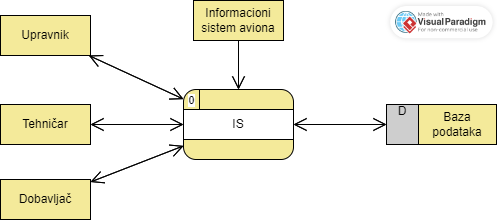
\includegraphics[scale=0.55]{Dijagrami/Dijagrami_toka_podataka/DTP_dijagram_konteksta.png}
\end{center}
\caption{Dijagram konteksta}
\label{fig:dtp_dijagram_konteksta}
\end{figure}

\begin{figure}[H]
\begin{center}
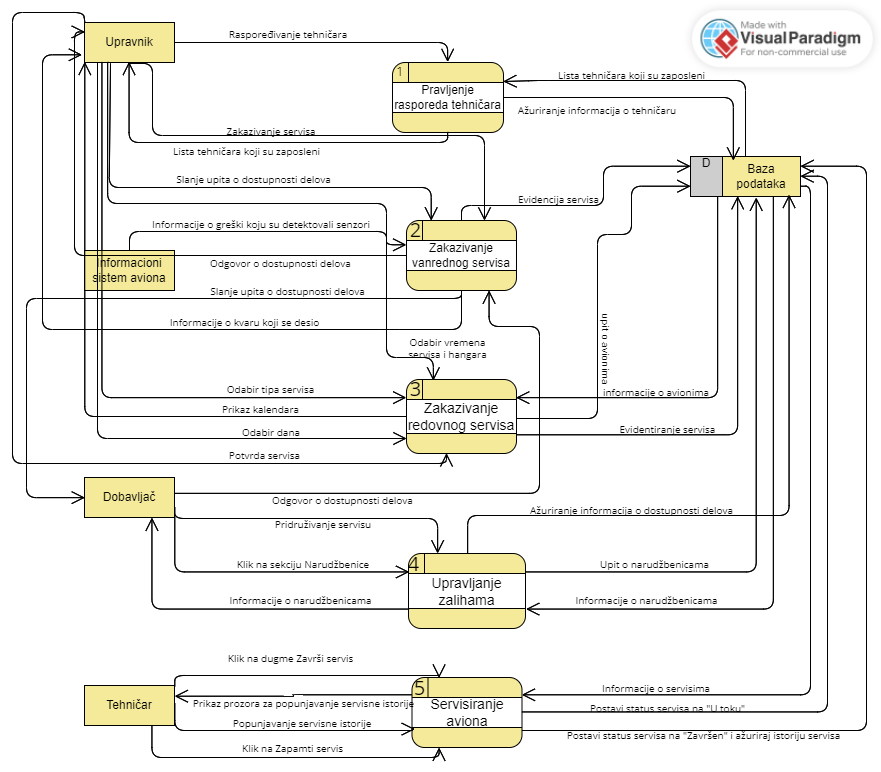
\includegraphics[scale=0.7, width = 1.1\textwidth]{Dijagrami/Dijagrami_toka_podataka/DTP_nivo_0.png}
\end{center}
\caption{Dijagram toka podataka nivoa 0}
\label{fig:dtp_nivoa_0}
\end{figure}

\section{Slučajevi upotrebe}
\label{sec:sluvajevi_upotrebe}
U ovom poglavlju ćemo detaljno opisati osnovne slučajeve upotrebe našeg sistema, pružajući uvid u ključne scenarije i funkcionalnosti koje naš sistem omogućava. Radi bolje preglednosti, nakon slučaja upotrebe celog sistema (slika \ref{fig:ceo_sistem}), ostali slučajevi upotrebe će biti grupisani na osnovu korisnika navedenih u glavi \ref{subsec:korisnici_sistema}.

\begin{figure}[H]
\begin{center}
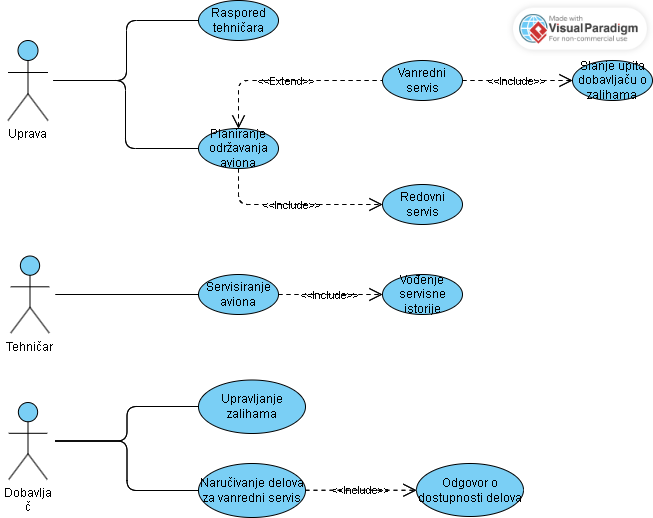
\includegraphics[scale=0.55]{Dijagrami/Dijagrami_slucajeva_upotrebe/Dijagram_slučajeva_upotrebe_celog_informacionog_sistema.png}
\end{center}
\caption{Dijagram slučajeva upotrebe celog informacionog sistema}
\label{fig:ceo_sistem}
\end{figure}

Radi boljeg razumevanja funkcionisanja celog sistema, ispod (Slika \ref{fig:bpmn_dijargram_saradnje}) je priložen dijagram saradnje izmedju upravnika i dobavljača.

\begin{figure}[H]
\begin{center}
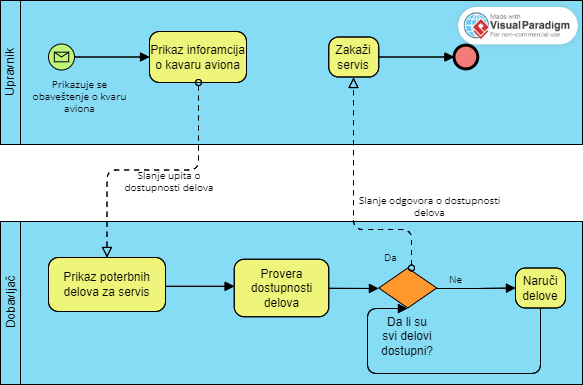
\includegraphics[scale=0.6]{Dijagrami/BPMN_Dijagrami/Dijagram_saradnje_upravnik_dobavljac.png}
\end{center}
\caption{Dijagram saradnje upravnika i dobavljača}
\label{fig:bpmn_dijargram_saradnje}
\end{figure}

\subsection{Slučaj upotrebe: Raspored tehničara}
\label{subsec:raspored_tehnicara}
\begin{itemize}
    \item \textbf{Kratak opis}: Sistem omogućava upravi da vidi dostupne tehničare, na osnovu čega se pravi raspored njihovog radnog vremena. Tehničari se raspoređuju u hangare. U svakom hangaru mora da bude raspoređeno minimalno 5 tehničara, a maksimalno 10. Smene traju 12 sati.
    \item \textbf{Akteri}: Upravnik
    \item \textbf{Preduslovi}: Sistem je aktivan i korisnik je prijavljen kao upravnik.
    \item \textbf{Postuslovi}: Raspored je napravljen i vidljiv svim tehničarima.
    \item \textbf{Osnovni tok}:
        \begin{enumerate}
            \item Klikom na sekciju $"$Raspored$"$ otvara se kalendar sa radnim danima u tom mesecu.
            \item Odabirom radnog dana otvara se prozor gde je potrebno uneti ID, ime i prezime, kao i radno vreme tehničara, i hangar u koji je tehničar raspoređen.
            \item Klikom na polje ID otvara mu se padajući meni sa svim podacima o dostupnim tehničarima u sistemu (ime, prezime, broj dodeljenih radnih sati, maksimalan broj radnih sati, minimalan broj radnih sati).
            \item Odabirom ID tehničara, sva polja iz 2. tačke se automatski popunjavaju, osim radnog vremena i hangara koje je potrebno eksplicitno navesti. Prvo se unosi radno vreme, a nakon toga se automatski nude hangari na kojim nema raspoređen dovoljan broj tehničara.
            \item Klikom na $"$Dodaj tehničara$"$, uneti tehničar se raspoređuje za izabrani dan. Broj radnih sati se automatski ažurira za izabranog tehničara.
        \end{enumerate}
    \item \textbf{Alternativni tokovi}:
        \begin{enumerate}
            A1) U slučaju da neki tehničar iznenada nije dostupan za neki period, potrebno je izmeniti raspored.
        \end{enumerate}
    \item \textbf{Specijalni uslovi}: Tehničar se ne može rasporediti ukoliko nije dostupan. Tehničar nije dostupan ukoliko mu je ispunjen maksimalan broj radnih sati za taj mesec ili ako je na odmoru/bolovanju. Tehničari vide raspored do poslednjeg popunjenog dana.
\end{itemize}

Slike \ref{fig:ds_raspored_tehnicara}. i \ref{fig:da_raspored_tehnicara} predstavljaju prateće dijagrame za ovaj slučaj upotrebe.
\begin{figure}[H]
\begin{center}
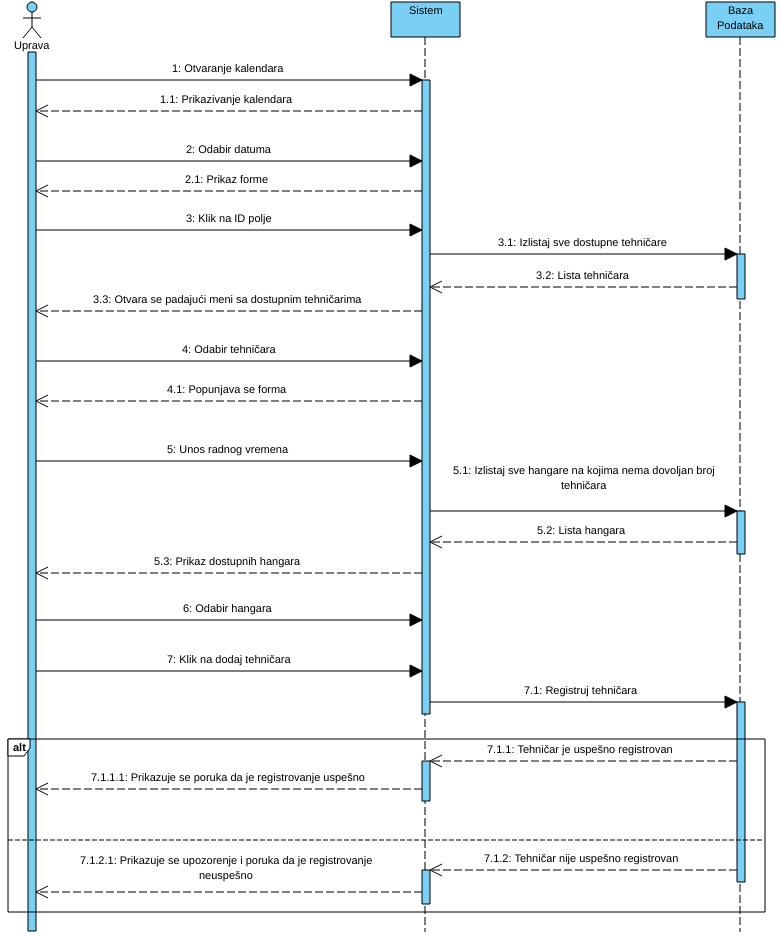
\includegraphics[scale=0.5, width = 1.1\textwidth]{Dijagrami/Dijagrami_sekvence/Dijagram_sekvence_rasporeda_tehničara.png}
\end{center}
\caption{Dijagram sekvence rasporeda tehničara}
\label{fig:ds_raspored_tehnicara}
\end{figure}

\begin{figure}[H]
\begin{center}
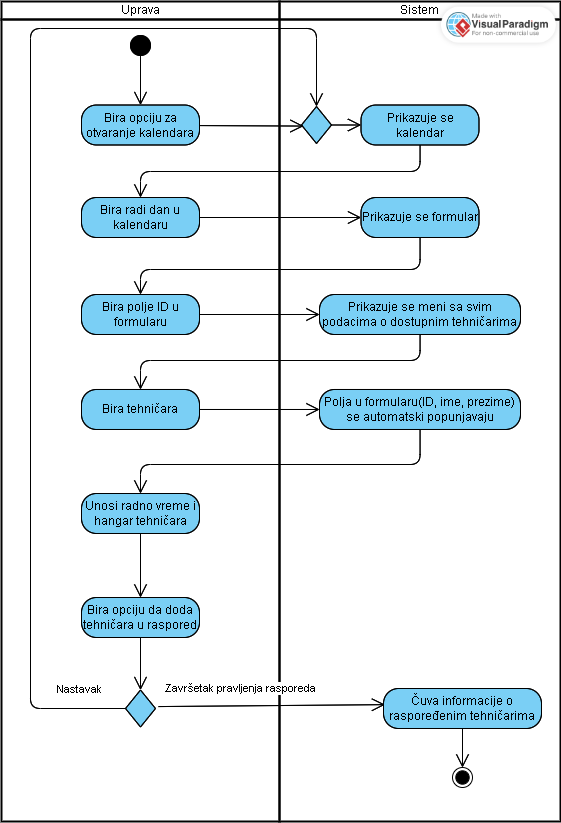
\includegraphics[scale=0.5]{Dijagrami/Dijagrami_aktivnosti/Dijagram_aktivnosti_raspored_tehničara.png}
\end{center}
\caption{Dijagram aktivnosti rasporeda tehničara}
\label{fig:da_raspored_tehnicara}
\end{figure}

\begin{figure}[H]
\begin{center}
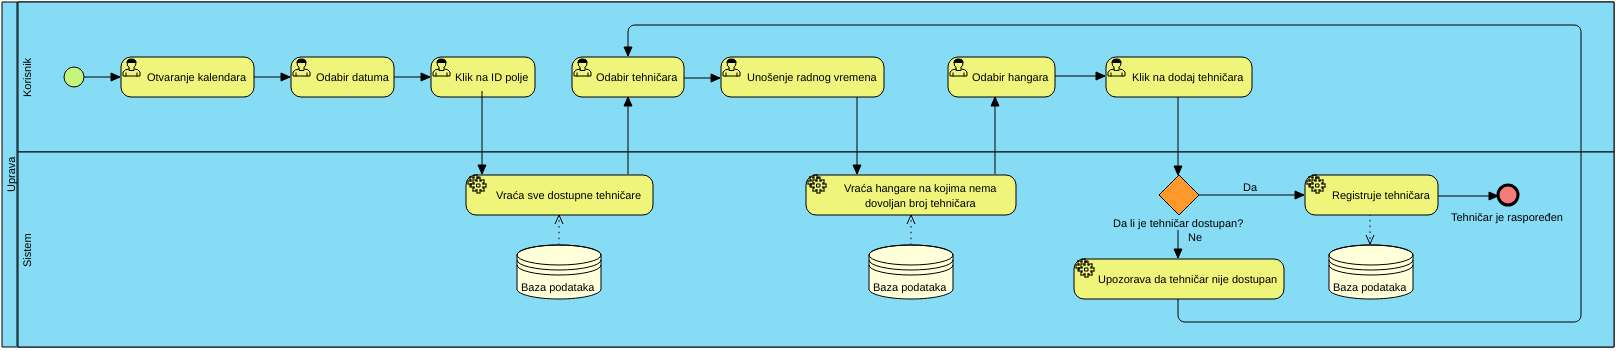
\includegraphics[scale=0.8, width = 1.3\textwidth]{Dijagrami/BPMN_Dijagrami/BPMN_rasporeda_tehničara.png}
\end{center}
\caption{BPMN dijagram - rasporeda tehničara}
\label{fig:da_raspored_tehnicara}
\end{figure}

\subsection{Slučaj upotrebe: Planiranje održavanja aviona - redovni servis}
\label{subsec:redovan_servis}
\begin{itemize}
    \item \textbf{Kratak opis}: Sistem omogućava upravi da pravi planove redovnih servisa aviona.
    \item \textbf{Akteri}: Upravnik
    \item \textbf{Preduslovi}: Sistem je aktivan, a korisnik je član uprave. Korisnik ima informacije o svim avionima.
    \item \textbf{Postuslovi}: Plan je napravljen. Tehničari vide plan održavanja. Dobavljači vide plan održavanja.
    \item \textbf{Osnovni tok}: 
    \begin{enumerate}
        \item Klikom na sekciju $"$Planiranje servisa$"$ otvara se meni sa svim avionima.

        \item Klikom na neki od aviona otvaraju se informacije o tom avionu kao što su proizvođač, model, godina proizvodnje, broj ciklusa motora od poslednjeg servisa, broj sati rada motora od poslednjeg servisa, datum poslednjeg dnevnog servisa, nedeljnog servisa i velikog servisa...

        \item Klikom na dugme $"$Zakaži servis$"$ mu se prikazuju tri opcije: $"$Dnevni servis$"$, $"$Nedeljni servis$"$ i $"$Veliki servis$"$ (na osnovu broja ciklusa motora ili radnih sati)
        \begin{enumerate}[label=3.1.\arabic*]
            \item Ukoliko je odabran $"$Dnevni servis$"$, on mora da bude zakazan u narednih 48 sati. Klikom na polje $"$Vreme servisa$"$ bira neki od slobodnih termina (avion nije na letu) u narednih 48 sati.
            \item Nakon što je odabrao termin (svaki dnevni servis traje 3h), dobija listu slobodnih hangara, klikom na polje $"$Hangar$"$, u izabrano vreme i opredeljuje se za jedan (na avionu rade tehničari koji su u to vreme raspoređeni u izabranom hangaru). Hangar se automatski rezerviše za odabrani period.
        \end{enumerate}
        \begin{enumerate}[label=3.2.\arabic*]
            \item Ukoliko je odabran $"$Nedeljni servis$"$, on može biti zakazan u narednih sedam dana. Klikom na polje $"$Vreme servisa$"$ bira neki od slobodnih termina (avion nije na letu) u narednih nedelju dana.
            \item Nakon što je odabrao termin (svaki nedeljni servis traje 6h), dobija listu slobodnih hangara, klikom na polje $"$Hangar$"$, u izabrano vreme i opredeljuje se za jedan (na avionu rade tehničari koji su u to vreme raspoređeni u izabranom hangaru). Hangar se automatski rezerviše za odabrani period.
        \end{enumerate}

         \begin{enumerate}[label=3.3.\arabic*]
            \item Klik na polje "Veliki servis" je moguć samo ukoliko je neki od parametara broj ciklusa motora ili broj sati rada motora blizu granice za servisiranje. Korisniku je automatski preporučen datum kada je predviđeno da se servis odradi. Trajanje servisa nije vremenski ograničeno.
            \item Klik na polje $"$Veliki servis$"$ je moguć samo ukoliko je neki od parametara broj ciklusa motora ili broj sati rada motora blizu granice za servisiranje. Korisniku je automatski preporučen datum kada je predviđeno da se servis odradi. Trajanje servisa nije vremenski ograničeno.
        \end{enumerate}
        \item Klikom na dugme $"$Potvrdi$"$, korisnik zakazuje servis.
        
    \end{enumerate}
    \item \textbf{Alternativni tokovi}:
        \begin{itemize}
        A1) Ukoliko je $"$hijerarhijski slabiji$"$ servis zakazan blizu $"$jačeg$"$ servisa, korisniku se nudi opcija da ga promoviše u jači. \\
        A2) Ukoliko odbije tu opciju, dobija poruku $"$Neuspešno zakazivanje servisa$"$.
        \end{itemize}
    \item \textbf{Specijalni uslovi}: Prilikom obavljanja $"$hijerarhijski jačeg$"$ servisa ažurira se i vreme servisa za sve slabije tipove servisa.
\end{itemize}

\subsection{Slučaj upotrebe: Planiranje održavanja aviona - vanredni servis}
\label{subsec:vanredni_servis}
\begin{itemize}
    \item \textbf{Kratak opis}: Sistem omogućava upravi da rukovodi vanrednim servisima aviona.
    \item \textbf{Akteri}: Upravnik
    \item \textbf{Preduslovi}: Sistem je u aktivnom stanju. Avion opremljen ispravnim senzorima koji funkcionišu. Ukoliko senzor detektuje grešku, sistem aviona je sposoban da prepozna tip greške i prenese informaciju ovom sistemu.
    \item \textbf{Postuslovi}: Vanredni servis je zakazan. Tehničari vide plan održavanja. Dobavljači vide plan održavanja.
    \item \textbf{Osnovni tok}:
    \begin{enumerate}
        \item Na ekranu je, u vidu prozora, prikazano obaveštenje o kvaru aviona. Klikom na dugme $"$Prikaži više$"$ otvaraju se detaljnije informacije o kvaru.
        \item Uprava klikom na dugme $"$Pošalji upit o rezervnim delovima$"$ šalje ove informacije o kvaru dobavljačima.
        \item Kada dobije odgovor o dostupnosti delova (od dobavljača), prikazuje mu se poruka u prozoru. Klikom na dugme $"$Zakaži servis$"$ koje se nalazi ispod poruke mu se otvara dijalog za zakazivanje servisa pokvarenom avionu.
        \item Polje vreme servisa je automatski popunjeno na prvi slobodan termin (u obzir se uzima i dostupnost potrebnih delova). Klikom na njega može da se i odabere neko drugo vreme.
        \item Kada se odabere vreme, klikom na polje $"$Hangar$"$ bira se neki od slobodnih hangara za odabrani termin.
        \item Klikom na dugme $"$Potvrdi$"$, korisnik zakazuje servis. Servis je dodat u plan održavanja.
    \end{enumerate}
    
    \item \textbf{Alternativni tokovi}:
        \begin{enumerate}
            A1) Ukoliko je vanredni servis zakazan $"$blizu$"$ dnevnog ili nedeljnog servisa ($\pm$1 dan), korisniku se nudi opcija da otkaže redovan servis.
        \end{enumerate}
    \item \textbf{Specijalni uslovi}: Prilikom obavljanja vanrednog servisa, ažuriraju se vremena za dnevni i nedeljni servis u bazi podataka.
\end{itemize}

Komunikacija koja se odvija sa dobavljačima je detaljno prikazana na slici \ref{fig:bpmn_dijargram_saradnje}.

\begin{figure}[H]
\begin{center}
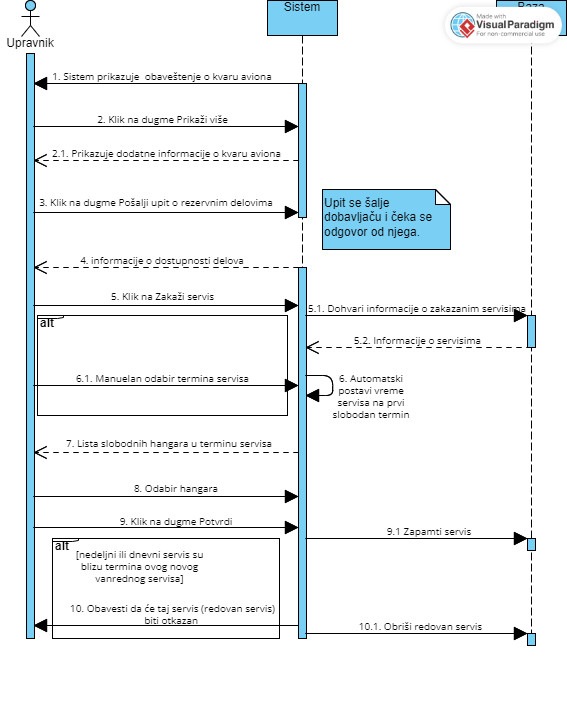
\includegraphics[scale=0.6, width = 1.0\textwidth]{Dijagrami/Dijagrami_sekvence/Dijagram_sekvence_zakazivanje_vanrednog_servisa.png}
\end{center}
\caption{Dijagram sekvence zakazivanja vanrednog servisa}
\label{fig:ds_zakazivanje_vanrednog_servisa}
\end{figure}


\begin{figure}[H]
\begin{center}
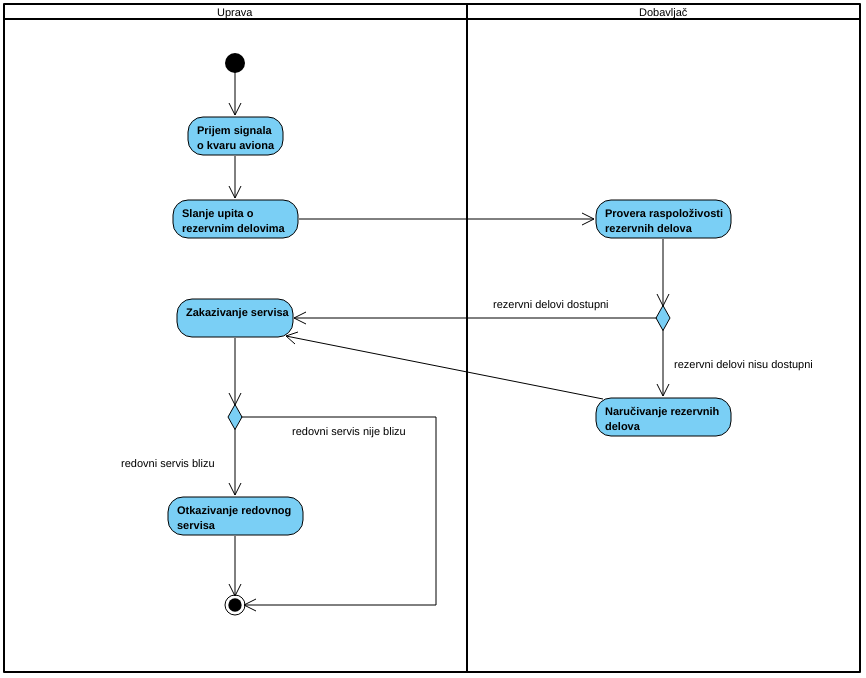
\includegraphics[scale=0.6, width = 1.0\textwidth]{Dijagrami/Dijagrami_aktivnosti/Dijagram_aktivnosti_vanrednog_servisa.png}
\end{center}
\caption{Dijagram aktivnosti zakazivanja vanrednog servisa}
\label{fig:da_zakazivanje_vanrednog_servisa}
\end{figure}

\subsection{Slučaj upotrebe - servisiranje aviona}
\label{subsec:servisiranje_aviona}
\begin{itemize}
    \item \textbf{Kratak opis}: Sistem omogućava tehničarima da vide raspored servisa i informacije o servisu. Tehničar servisira onaj avion čiji je servis zakazan za vreme njegovog radnog vremena u hangaru u kom je on raspoređen.
    \item \textbf{Akteri}: Tehničar
    \item \textbf{Preduslovi}: Sistem je aktivan. Raspored servisa je napravljen i dostupan tehničarima.
    \item \textbf{Postuslovi}: Serviser je uspešno obavio servis aviona i uneo servis u evidenciju.
    \item \textbf{Osnovni tok}:
        \begin{enumerate}
            \item Tehničar klikom na sekciju $"$Raspored servisa$"$ vidi sve zakazane servise. Klikom na određen servis vidi dodatne informacije za taj servis (tip aviona, proizvođač, godina, uputstva od proizvođača).
            \item Kada dođe vreme za određen servis, sistem automatski postavlja status servisa na $"$U toku$"$.
            \item Kada je servis završen, klikom na dugme $"$Završi servis$"$ otvara se prozor u kome treba da unese informacije o servisu koje će biti sačuvane kao servisna istorija aviona.
            \item U polju $"$Urađeno na servisu$"$ navodi sve što je urađeno u tom servisu. Polja kao što su tip servisa, datum i vreme servisa su unapred popunjena.
            \item Klikom na dugme $"$Zapamti servis$"$, servis se čuva u servisnoj istoriji i status mu je promenje u $"$Završen$"$.
        \end{enumerate}
    \item \textbf{Alternativni tokovi:}
        \begin{enumerate}
            A1) Ako je polje $"$Uradjeno na servisu$"$ prazno, a klikne se na dugme $"$Zapamti servis$"$, dobija se poruka o grešci.
        \end{enumerate}
    \item \textbf{Specijalni uslovi}: /
\end{itemize}

\begin{figure}[H]
\begin{center}
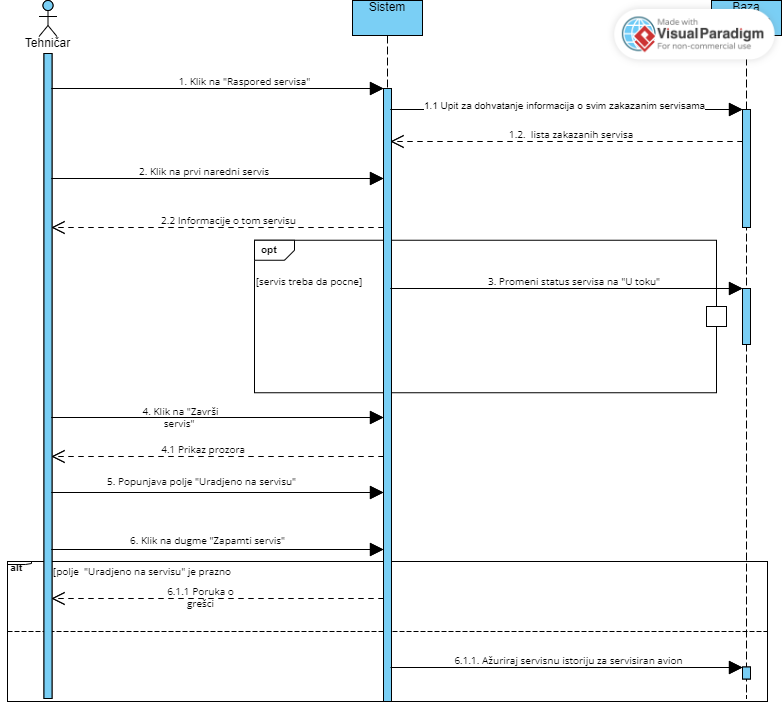
\includegraphics[scale=0.6, width = 1.0\textwidth]{Dijagrami/Dijagrami_sekvence/Dijagram_sekvence_servisiranje_aviona.png}
\end{center}
\caption{Dijagram sekvence servisiranja aviona}
\label{fig:ds_servisiranje_aviona}
\end{figure}

\subsection{Slučaj upotrebe - upravljanje zalihama}
\label{subsec:redovan_servis}
\begin{itemize}
    \item \textbf{Kratak opis}: Ovaj slučaj upotrebe fokusira se na upravljanje zalihama delova za avion od strane dobavljača, kako bi se osigurala dostupnost potrebnih komponenti za redovna servisiranja aviona. Sistem za automatsko nabavljenje delovima osmišljen je za praćenje, upravljanje i obezbeđivanje delova potrebnih za redovne servise.
    \item \textbf{Akteri}: Dobavljač
    \item \textbf{Preduslovi}: Postojanje sistema za automatsko upravljanje delovima. Dobavljač vidi rasporedu redovnih servisa i informacije o trenutnom stanju zaliha. Sistem je aktivan.
    \item \textbf{Postuslovi}: Ažurirane informacije o zalihama za sve redovne servise. U Rasporedu servisa je oznaceno da su delovi za taj servis spremni.
    \item \textbf{Osnovni tok}:
        \begin{enumerate}
            \item Klikom na sekciju $"$Narudžbine$"$ prikazuju mu se sve narudžbenice koje je sistem za automatsko upravljanje napravio.
            \item Klikom na narudžbenicu prikazuju mu se sve informacije o njoj (status narudžbenice, servis za koji je napravljena, vreme stizanja, informacije o naručenom delu itd...).
            \item Ukoliko je status narudžbenice $"$Isporučena$"$, dostupno mu je dugme $"$Pridruži servisu$"$. Klikom na dugme, delovi se automatski pridružuju servisu za koji su namenjeni i stanje delova se ažurira.
        \end{enumerate}
    \item \textbf{Alternativni tokovi}: /
    \item \textbf{Specijalni uslovi}: Sistem mora pružati tačne i ažurirane informacije o dostupnosti delova. Informacije o narudžbenicama moraju biti transparentne, uključujući procenjeni datum dolaska delova.
\end{itemize}

\begin{figure}[H]
\begin{center}
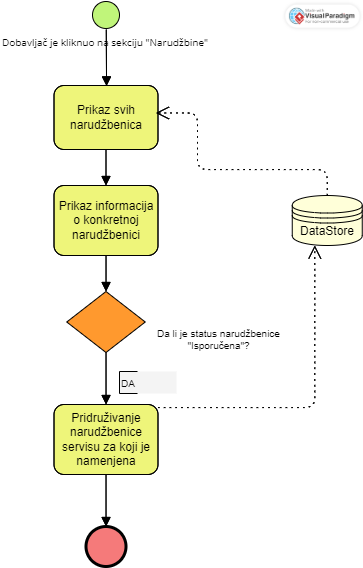
\includegraphics[scale=0.5]{Dijagrami/BPMN_Dijagrami/BPMN_dijagram_procesa_upravljanje_narudzbenicama.png}
\end{center}
\caption{Dijagram procesa - Upravljanje zalihama}
\label{fig:BPMN_upravljanje_zalihama}
\end{figure}

\subsection{Slučaj upotrebe - naručivanje delova za vanredni servis}
\label{subsec:narucivanje_vanredan_servis}
\begin{itemize}
    \item \textbf{Kratak opis}: Ovaj slučaj upotrebe pokriva naručivanje delova kada dođe do kvara aviona.
    \item \textbf{Akteri}: Dobavljač
    \item \textbf{Preduslovi}: Sistem funkcioniše. Uprava je dobila obaveštenje o kvaru aviona (sa informacijama o tome šta je pokvareno) i poslala upit dobavljaču o dostupnosti delova.
    \item \textbf{Postuslovi}: Uprava je obaveštena o dostupnosti delova (da li je deo dostupan ili očekivano vreme isporuke).
    \item \textbf{Osnovni tok}: 
        \begin{enumerate}
            \item Stiže obaveštenje od uprave da je došlo do kvara aviona. Klikom na obaveštenje dobijaju se informacije o pokvarenim delovima.
            \item Klikom na dugme $"$Proveri dostupnost$"$, dobavljač dobija informaciju o dostupnosti datih delova.
            \item Ukoliko su svi delovi dostupni, omogućeno mu je da odmah pošalje odgovor upravi da su svi potrebni delovi dostupni, klikom na dugme $"$Pošalji odgovor$"$.
            \item Ukoliko neki deo nije dostupan, pored njega postoji dugme $"$Naruči deo$"$. Klikom na ovo dugme sistem za automatsko naručivanje se pokreće i pravi narudžbenicu. Kada sistem naruči deo, dobija potvrdu.
            \item Kada su svi delovi ili dostupni ili naručeni, moguće je da klikne na dugme $"$Pošalji odgovor$"$, čime šalje odgovor upravi o dostupnosti delova (odgovor sadrži informacije o dostupnosti delova; da li je deo dostupan ili procenjeno vreme dolaska).
        \end{enumerate}
    \item \textbf{Alternativni tokovi}: /
    \item \textbf{Specijalni uslovi}: Sistem mora pružati tačne i ažurirane informacije o dostupnosti delova. Informacije o narudžbenicama moraju biti transparentne, uključujući procenjeni datum dolaska delova.
\end{itemize}

Komunikacija koja se odvija sa upravnikom je detaljno prikazana na slici \ref{fig:bpmn_dijargram_saradnje}.
\begin{figure}[H]
\begin{center}
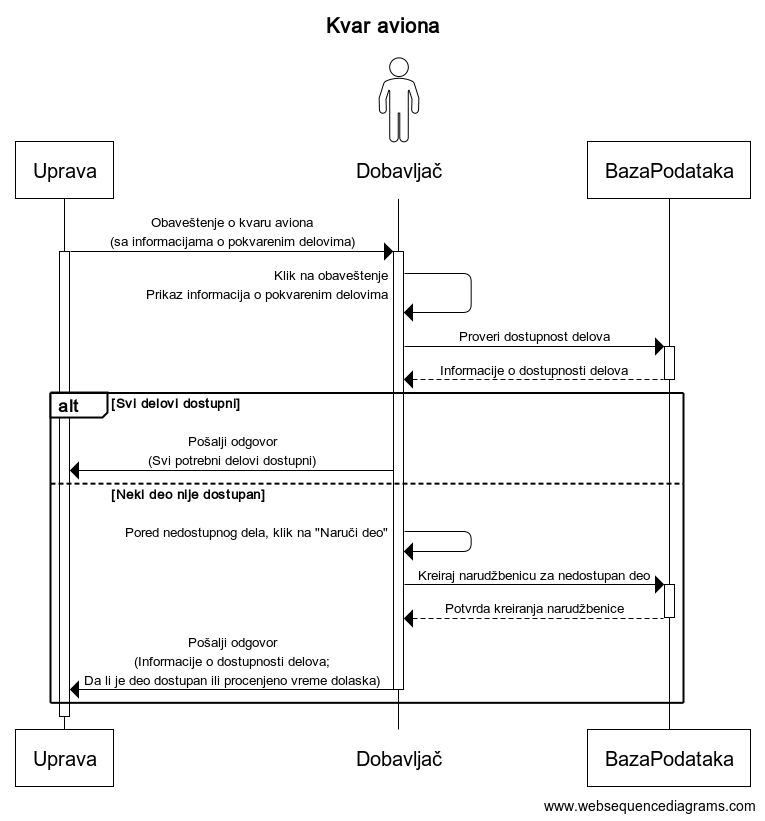
\includegraphics[scale=0.4]{Dijagrami/Dijagrami_sekvence/Dijagram_sekvenci_narucivanje_delova.png}
\end{center}
\caption{Dijagram sekvence naručivanja delova}
\label{fig:ds_narucivanje_delova}
\end{figure}

\section{Zaključak}
\label{sec:zakljucak}

Ovde pišem zaključak. 
Ovde pišem zaključak. 
Ovde pišem zaključak. 
Ovde pišem zaključak. 
Ovde pišem zaključak. 
Ovde pišem zaključak. 
Ovde pišem zaključak. 
Ovde pišem zaključak. 
Ovde pišem zaključak. 
Ovde pišem zaključak. 
Ovde pišem zaključak. 
Ovde pišem zaključak. 


\addcontentsline{toc}{section}{Literatura}
\appendix
\bibliography{seminarski} 
\bibliographystyle{plain}

\appendix
\section{Dodatak}
Ovde pišem dodatne stvari, ukoliko za time ima potrebe.
Ovde pišem dodatne stvari, ukoliko za time ima potrebe.
Ovde pišem dodatne stvari, ukoliko za time ima potrebe.
Ovde pišem dodatne stvari, ukoliko za time ima potrebe.
Ovde pišem dodatne stvari, ukoliko za time ima potrebe.


\end{document}
